\chapter{Estructura social y castas}

\begin{figure}[t]
\centering
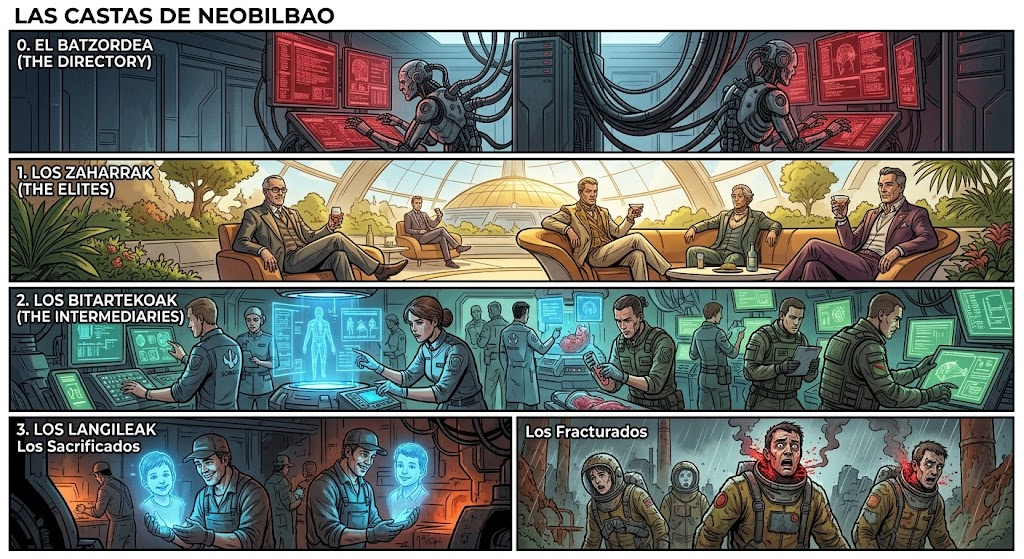
\includegraphics[width=0.95\linewidth]{castas.png}
\caption{La pirámide social de NeoBilbao: Directorio, elites, intermediarios y obreros.}
\end{figure}

\section{El Directorio (Batzordea)}

Por encima de toda la sociedad se sienta el Batzordea, un puñado de individuos reunidos en torno a los fundadores de Orekak-Corp y a los ingenieros jefe de Ibaizabal-Burdin. Son ancianos mantenidos mediante cibernética extrema, desconectados de la humanidad.

\textbf{Nivel de conocimiento:} total y absoluto. Saben que la Cúpula Dorada se sostiene con los cerebros de los niños, y que el Velo es un sistema de anestesia emocional diseñado para mantener a la manufactura obrera bajo control. Para ellos, la colonia es una ecuación. El dolor es un coste calculado.

\section{Casta alta: los Zaharrak}

Los Zaharrak son los descendientes de los primeros oficiales de la flota y de los ejecutivos corporativos. Viven en la zona más protegida de la Cúpula, donde el aire es limpio, la luz es artificial y el tiempo es un lujo que no conocen. Sus vidas están rodeadas de jardines sintéticos, módulos de confort y alteraciones genéticas de prestigio.

\textbf{Nivel de conocimiento:} ignorancia cómoda y ceguera voluntaria. No saben que los niños de los Zócalos son usados como máquinas orgánicas ni que el Velo es una simulación propagandística. Creen la narrativa oficial: los obreros son necesarios, los niños están seguros en internados corporativos y el Velo es un incentivo benevolente.

\section{Casta media: los Bitartekoak}

Los Bitartekoak forman la burocracia, la seguridad de rango medio, los técnicos de mantenimiento y el Círculo Médico. Viven en el anillo inferior de la Cúpula, donde el aire es limpio y la vida es más gris y menos privilegiada.

\textbf{Nivel de conocimiento:} parcial, fragmentado y traumático. Estos personajes observan piezas sueltas del horror:
\begin{itemize}
  \item Los técnicos informáticos saben que la energía del sistema se basa en un hardware orgánico inestable.
  \item Los capataces del basajaun conocen el Velo como una herramienta de manipulación emocional, pero creen que las «videollamadas» son reales.
  \item El Círculo Médico conoce la extracción de niños y su conexión a los tanques, pero su memoria es fragmentada por amnésicos y lavado de cerebro.
\end{itemize}

\section{Casta baja: los Langileak}

La masa obrera de los Zócalos Industriales vive bajo la lluvia ácida y la sombra de los hornos. En la práctica, su condición social es perpetua: trabajan, consumen y obedecen, mientras los demás disfrutan de la luz superior.

\subsection*{Los Sacrificados}

El 90\% de la población cree de verdad que el Etxearen Zina es un sacrificio justo. Su dolor se ha convertido en una forma de amor. No son conscientes del horror real. Piensan que sus hijos están seguros, educados, felices y protegidos por la corporación.

\subsection*{Los Fracturados}

El 10\% restante son los obreros a los que se les ha cortado o dañado el Velo. Son los primeros en darse cuenta de la mentira. Descubren la estática, las anomalías y la corrupción del sistema, abierto paso a la resistencia. No saben todavía la verdad completa, pero ya no pueden volver a la ilusión.

\textbf{Regla de la campaña:} la percepción del mundo depende del conocimiento. Los personajes no solo se mueven por la física del planeta, sino por la estructura moral de la colonia. El horror se inscribe al nivel del lenguaje, la compulsión y el engaño.
